\documentclass[11pt,a4paper]{report}

\usepackage[spanish,es-tabla]{babel}
\usepackage[utf8]{inputenc}
\usepackage[T1]{fontenc}
\usepackage{lmodern}
\usepackage[a4paper,margin=2.5cm]{geometry}
\usepackage{amsmath}
\usepackage{booktabs}
\usepackage{array}
\usepackage{graphicx}
\usepackage{float}
\usepackage{caption}
\usepackage{subcaption}
\usepackage{xcolor}
\usepackage{hyperref}
\usepackage{pgfplots}

\pgfplotsset{compat=1.18}
\graphicspath{{figuras_memoria/}}

\title{Memoria parcial de clasificaci\'on de artefactos arqueol\'ogicos}
\author{Proyecto de clasificaci\'on de artefactos arqueol\'ogicos}
\date{\today}

\begin{document}

\maketitle

\begin{abstract}
Este documento resume dos bloques experimentales del proyecto. El primero compara tres arquitecturas ligeras para clasificaci\'on de artefactos arqueol\'ogicos: una CNN directa sobre imagen, una MLP alimentada por un VAE y una KAN tambi\'en alimentada por un VAE. El segundo estudia una estrategia de \textit{transfer learning} con \texttt{EfficientNet-B0} y compara dos posibles cabezas finales, una MLP y una KAN. En ambos casos la base experimental es el \texttt{cssl\_dataset}.
\end{abstract}

\tableofcontents

\chapter{Modelos ligeros: CNN, VAE + MLP y VAE + KAN}

\section{Objetivo del experimento}

El objetivo de este bloque es comparar tres formas distintas de resolver la misma tarea de clasificaci\'on:

\begin{itemize}
    \item una arquitectura visual directa, especializada en explotar la estructura espacial de la imagen (CNN);
    \item una arquitectura densa que trabaja sobre una representaci\'on latente comprimida (VAE + MLP);
    \item una arquitectura alternativa a la MLP, tambi\'en sobre espacio latente, pero con capas KAN basadas en expansiones RBF (VAE + KAN).
\end{itemize}

La hip\'otesis de partida era que el espacio latente aprendido por el VAE pod\'ia facilitar la clasificaci\'on en problemas visuales modestos, y que una cabeza KAN podr\'ia capturar relaciones no lineales m\'as expresivas que una MLP convencional.

\section{Dataset utilizado}

Los experimentos se han realizado sobre el conjunto \texttt{cssl\_dataset}, en la tarea de clasificaci\'on por forma contenida en:

\begin{center}
\texttt{cssl\_dataset/experiments/regular\_shape/shapes/train\_sets}
\end{center}

El dataset contiene dos modalidades:

\begin{itemize}
    \item \texttt{photos}: fotograf\'ias de artefactos;
    \item \texttt{drawings}: dibujos o representaciones esquem\'aticas de esos artefactos.
\end{itemize}

Las clases usadas en este bloque son diez:

\begin{center}
\texttt{ankh, anthropomorphic, bands, beetle, bird, circles, cross, ibex, lion, sa}
\end{center}

En todos los casos las im\'agenes se leen en escala de grises y se redimensionan a $256\times256$. Durante entrenamiento se aplica una aumentaci\'on ligera basada en \textit{horizontal flip} con probabilidad $0.5$ y una rotaci\'on aleatoria de hasta $8^\circ$. Tras ello, la entrada se normaliza con media $0.5$ y desviaci\'on t\'ipica $0.5$.

\subsection{Experimentos analizados}

En esta memoria se recogen los resultados que ya estaban entrenados y almacenados en \texttt{CNN\_ARTEFACTOS/checkpoints} e \texttt{CNN\_ARTEFACTOS/historial}. En concreto, se han utilizado dos escenarios:

\begin{table}[H]
\centering
\caption{Configuraci\'on de los experimentos analizados.}
\resizebox{\textwidth}{!}{%
\begin{tabular}{>{\raggedright\arraybackslash}p{3.2cm} >{\raggedright\arraybackslash}p{2.3cm} c c c}
\toprule
Modalidad & Split & Tama\~no original & Muestras usadas & \'Epocas observadas \\
\midrule
Drawings & \texttt{50-50 / experiment\_0} & $507$ train / $513$ test & $400$ train / $200$ test & $20$ \\
Photos & \texttt{50-50-q / experiment\_0} & $129$ train / $513$ test & $129$ train / $200$ test & $50$ \\
\bottomrule
\end{tabular}
}
\end{table}

Es importante remarcar que el m\'odulo \texttt{CNN\_ARTEFACTOS} est\'a dise\~nado como versi\'on ligera del proyecto. Por defecto limita el n\'umero de ejemplos a \texttt{400} en entrenamiento y \texttt{200} en validaci\'on/test para abaratar el coste computacional. Por tanto, la comparaci\'on principal es v\'alida dentro de cada experimento, pero no debe interpretarse como una comparaci\'on directa entre dibujos y fotograf\'ias, ya que cambian tanto la modalidad como el split.

\section{Arquitecturas evaluadas}

\subsection{CNN directa sobre imagen}

La arquitectura \texttt{SmallArtefactCNN} recibe la imagen en escala de grises y la procesa directamente mediante cuatro bloques convolucionales. El n\'umero de canales evoluciona como
\[
1 \rightarrow 16 \rightarrow 32 \rightarrow 64 \rightarrow 96.
\]

Cada bloque utiliza dos convoluciones $3\times3$, normalizaci\'on \texttt{BatchNorm2d} y activaci\'on \texttt{ReLU}, con operaciones de \texttt{MaxPool2d} entre bloques. Al final se aplica una agregaci\'on global mediante \texttt{AdaptiveAvgPool2d} y una peque\~na cabeza densa
\[
96 \rightarrow 64 \rightarrow 10.
\]

Esta red sirve como baseline, ya que conserva la estructura espacial de la imagen durante casi todo el pipeline y aprende directamente patrones locales de borde, textura y forma.

\subsection{VAE compartido para MLP y KAN}

Las arquitecturas MLP y KAN no clasifican la imagen original directamente. Antes de clasificar, ambas pasan por un VAE ligero. Su encoder est\'a formado por tres capas convolucionales estriadas, con progresi\'on
\[
1 \rightarrow 16 \rightarrow 32 \rightarrow 48.
\]

Sobre esa representaci\'on se estiman $\mu$ y $\log\sigma^2$, se aplica la reparametrizaci\'on gaussiana y, finalmente, un decoder con convoluciones transpuestas intenta reconstruir la imagen de entrada. El encoder produce un mapa latente de tama\~no $1 \times 32 \times 32$, equivalente a 1024 caracter\'isticas tras aplicar \textit{flatten}. La idea es sustituir la imagen cruda por una representaci\'on m\'as compacta antes de clasificar.

\subsection{Clasificador VAE + MLP}

La red \texttt{SmallArtefactMLP} toma el latente $32\times32$, lo aplana y lo clasifica con una MLP de tres capas densas:
\[
1024 \rightarrow 256 \rightarrow 128 \rightarrow 10.
\]

Las dos capas ocultas usan activaci\'on \texttt{ReLU} y \texttt{Dropout} de 0.25 y 0.15, respectivamente. En consecuencia, la tarea visual se transforma en una clasificaci\'on sobre un vector latente aprendido por el VAE.

\subsection{Clasificador VAE + KAN}

La red \texttt{SmallArtefactKAN} comparte el mismo VAE anterior, pero sustituye la MLP por una cabeza de clasificaci\'on basada en capas KAN:
\[
1024 \rightarrow 96 \rightarrow 48 \rightarrow 10.
\]

Las dos capas ocultas son \texttt{RBFKANLayer}, separadas por activaciones \texttt{SiLU} y un \texttt{Dropout} de 0.15. Cada capa KAN combina una parte lineal convencional con una expansi\'on no lineal basada en funciones base radiales sobre una rejilla aprendible. La motivaci\'on es disponer de una no linealidad m\'as estructurada que la de una capa densa est\'andar.

\section{Entrenamiento}

Los tres modelos se entrenan con optimizador \texttt{Adam}, tasa de aprendizaje inicial $10^{-3}$, \texttt{weight decay} de $10^{-4}$ y \texttt{batch size} de 16. En todos los casos se conserva como checkpoint final el estado correspondiente a la mejor \texttt{val\_acc}.

La funci\'on de p\'erdida no es exactamente la misma para todos los modelos:

\begin{equation}
\mathcal{L}_{\text{CNN}} = \mathcal{L}_{\text{CE}}
\end{equation}

\begin{equation}
\mathcal{L}_{\text{MLP/KAN}} = \mathcal{L}_{\text{CE}} + 0.35\,\mathcal{L}_{\text{recon}} + 0.02\,\mathcal{L}_{\text{KL}}
\end{equation}

donde $\mathcal{L}_{\text{CE}}$ es la entrop\'ia cruzada de clasificaci\'on, $\mathcal{L}_{\text{recon}}$ es el error de reconstrucci\'on del VAE y $\mathcal{L}_{\text{KL}}$ es la regularizaci\'on KL del espacio latente.

Esto tiene una consecuencia importante a la hora de interpretar las figuras: la accuracy s\'i es comparable entre modelos, pero la loss total no debe compararse de forma absoluta entre CNN y los modelos con VAE, porque en MLP/KAN incorpora t\'erminos extra que la CNN no tiene.

\section{Resultados obtenidos}

\subsection{Resultados sobre drawings}

La comparaci\'on principal m\'as limpia es la de \texttt{drawings / 50-50 / experiment\_0}, donde se entrenaron las tres arquitecturas en el mismo contexto experimental.

\begin{table}[H]
\centering
\caption{Mejor resultado de validaci\'on sobre \texttt{drawings / 50-50 / experiment\_0}.}
\resizebox{0.82\textwidth}{!}{%
\begin{tabular}{lcccc}
\toprule
Modelo & Mejor \'epoca & Train acc. & Val acc. & Gap train-val \\
\midrule
CNN & 20 & 0.3000 & 0.2250 & 0.0750 \\
MLP & 18 & 0.9417 & 0.3500 & 0.5917 \\
KAN & 18 & 0.8750 & 0.3417 & 0.5333 \\
\bottomrule
\end{tabular}
}
\end{table}

La lectura de estos resultados es clara:

\begin{itemize}
    \item la MLP obtiene la mejor accuracy de validaci\'on (0.3500);
    \item la KAN queda muy cerca (0.3417);
    \item la CNN queda bastante por debajo (0.2250).
\end{itemize}

En este escenario, trabajar sobre un espacio latente aprendido por el VAE resulta m\'as eficaz que clasificar el dibujo directamente con una CNN peque\~na. Sin embargo, tanto la MLP como la KAN muestran un gap grande entre train y validaci\'on, lo que sugiere sobreajuste. La MLP logra una validaci\'on ligeramente mejor, pero tambi\'en sobreajusta algo m\'as que la KAN.

\begin{figure}[H]
\centering
\begin{subfigure}[t]{0.48\textwidth}
    \centering
    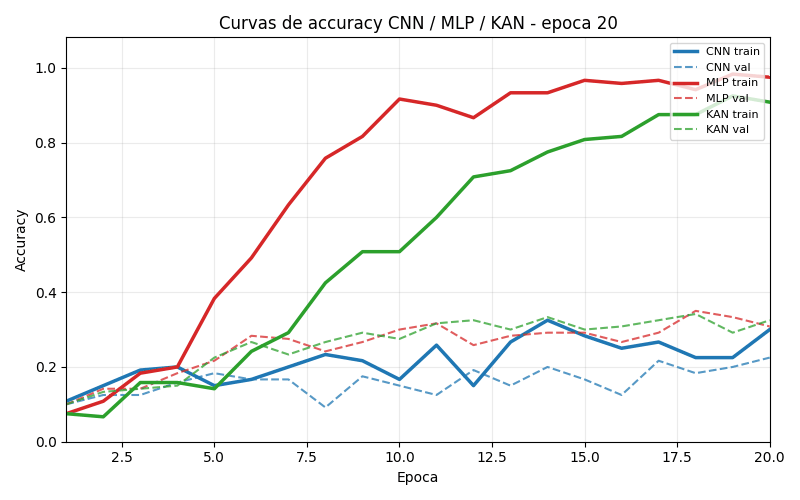
\includegraphics[width=\linewidth]{comparacion_accuracy_drawings_50-50_experiment_0.png}
    \caption{Curvas de accuracy.}
\end{subfigure}
\hfill
\begin{subfigure}[t]{0.48\textwidth}
    \centering
    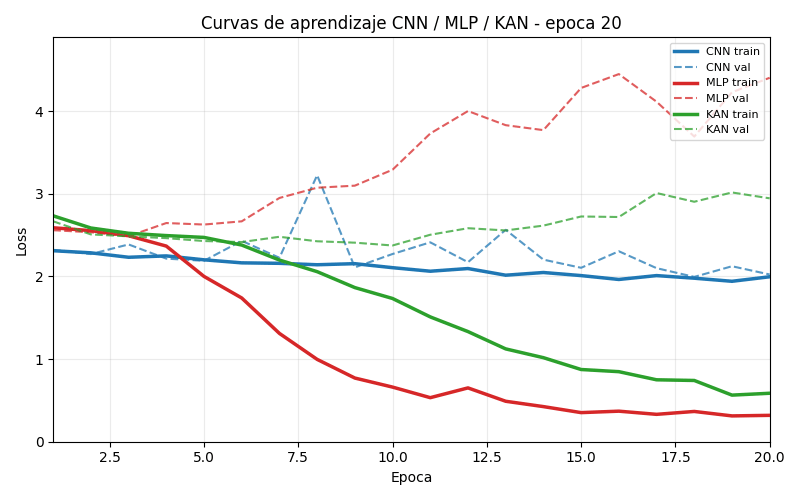
\includegraphics[width=\linewidth]{comparacion_loss_drawings_50-50_experiment_0.png}
    \caption{Curvas de loss total.}
\end{subfigure}
\caption{Evoluci\'on del entrenamiento en el experimento con dibujos. Las curvas se han extra\'ido de los GIFs generados por el propio m\'odulo \texttt{CNN\_ARTEFACTOS}.}
\end{figure}

\subsection{Resultados sobre photos}

Como complemento, tambi\'en se dispone de un segundo experimento sobre \texttt{photos / 50-50-q / experiment\_0}. En este caso la cantidad de entrenamiento es mucho menor, ya que el split original solo contiene 129 muestras de train.

\begin{table}[H]
\centering
\caption{Mejor resultado de validaci\'on sobre \texttt{photos / 50-50-q / experiment\_0}.}
\resizebox{0.82\textwidth}{!}{%
\begin{tabular}{lcccc}
\toprule
Modelo & Mejor \'epoca & Train acc. & Val acc. & Gap train-val \\
\midrule
CNN & 50 & 0.5659 & 0.2400 & 0.3259 \\
MLP & 44 & 0.8605 & 0.2000 & 0.6605 \\
KAN & 24 & 0.2248 & 0.1500 & 0.0748 \\
\bottomrule
\end{tabular}
}
\end{table}

En fotograf\'ias el patr\'on cambia:

\begin{itemize}
    \item la CNN es la mejor (0.2400);
    \item la MLP queda por debajo (0.2000);
    \item la KAN es la peor (0.1500).
\end{itemize}

Aqu\'i parece que el VAE no consigue construir una representaci\'on latente suficientemente robusta para mejorar la clasificaci\'on. Una explicaci\'on plausible es que, con tan pocas fotograf\'ias de entrenamiento, la compresi\'on previa del VAE introduce una dificultad adicional en lugar de ayudar. La CNN, aunque modesta, aprovecha mejor la estructura espacial directa de la imagen.

\subsection{Comparaci\'on visual resumida}

La Figura~\ref{fig:barras-resumen} resume la mejor \texttt{val\_acc} observada para cada modelo en los dos escenarios disponibles.

\begin{figure}[H]
\centering
\begin{tikzpicture}
\begin{axis}[
    ybar,
    bar width=12pt,
    width=0.9\textwidth,
    height=7cm,
    ymin=0,
    ymax=0.4,
    ylabel={Mejor accuracy de validaci\'on},
    symbolic x coords={CNN,MLP,KAN},
    xtick=data,
    legend style={at={(0.5,1.05)}, anchor=south, legend columns=2},
    nodes near coords,
    nodes near coords align={vertical},
    grid=major,
]
\addplot coordinates {(CNN,0.2250) (MLP,0.3500) (KAN,0.3417)};
\addplot coordinates {(CNN,0.2400) (MLP,0.2000) (KAN,0.1500)};
\legend{Drawings 50-50, Photos 50-50-q}
\end{axis}
\end{tikzpicture}
\caption{Resumen de la mejor accuracy de validaci\'on por modelo y escenario.}
\label{fig:barras-resumen}
\end{figure}

\section{Discusi\'on}

De los resultados anteriores se pueden extraer varias conclusiones relevantes:

\begin{enumerate}
    \item No existe un ganador universal. El comportamiento depende de la modalidad y del tama\~no efectivo del entrenamiento.
    \item En dibujos, el espacio latente del VAE s\'i ayuda. Tanto MLP como KAN superan claramente a la CNN.
    \item En fotograf\'ias, la CNN es m\'as estable. Cuando el conjunto de entrenamiento es peque\~no, la ruta directa sobre imagen parece m\'as robusta que introducir un VAE previo.
    \item KAN no mejora a MLP en los experimentos realizados. En dibujos queda muy cerca, pero no la supera; en fotograf\'ias queda claramente por debajo.
    \item MLP y KAN muestran sobreajuste. Los gaps entre accuracy de entrenamiento y de validaci\'on son altos, sobre todo en la MLP.
\end{enumerate}

En consecuencia, la conclusi\'on experimental de esta primera fase no es que KAN sea mejor que MLP, sino que la utilidad de la cabeza de clasificaci\'on depende del tipo de representaci\'on y del r\'egimen de datos. En nuestro caso, la KAN es una alternativa interesante, pero todav\'ia no aporta una mejora emp\'irica clara frente a la MLP est\'andar.

\section{Conclusi\'on del primer bloque}

Este primer bloque de trabajo ha servido para construir un marco de comparaci\'on sencillo y reutilizable sobre el dataset arqueol\'ogico. La comparaci\'on entre CNN, VAE + MLP y VAE + KAN permite estudiar tres filosof\'ias distintas:

\begin{itemize}
    \item aprendizaje visual directo sobre la imagen;
    \item clasificaci\'on densa sobre un espacio latente comprimido;
    \item clasificaci\'on sobre ese mismo espacio latente usando capas KAN.
\end{itemize}

Los resultados muestran que:

\begin{itemize}
    \item para \texttt{drawings}, la mejor opci\'on ha sido MLP, seguida muy de cerca por KAN;
    \item para \texttt{photos}, la mejor opci\'on ha sido la CNN;
    \item la KAN no ha superado a la MLP en los experimentos ya completados.
\end{itemize}

Por tanto, esta primera fase deja una conclusi\'on prudente pero valiosa: las capas KAN son prometedoras como alternativa, pero en este proyecto no han demostrado una ventaja consistente frente a una MLP convencional cuando se trabaja con modelos ligeros y con un VAE intermedio.

\chapter{Transfer learning con EfficientNet y comparaci\'on entre MLP y KAN}

\section{Objetivo y planteamiento}

En el segundo bloque se abandonan las arquitecturas ligeras del primer experimento y se pasa a un esquema de \textit{transfer learning}. La idea es aprovechar un backbone visual preentrenado, \texttt{EfficientNet-B0}, y comparar dos maneras de especializar su bloque final: una cabeza MLP convencional y una cabeza KAN. A diferencia del bloque anterior, aqu\'i la entrada no es una sola imagen, sino un par formado por una fotograf\'ia y un dibujo del mismo artefacto.

\section{Dataset y configuraci\'on experimental}

El experimento se ha realizado sobre el split \texttt{80-20 / experiment\_0} del mismo problema de clasificaci\'on por forma del \texttt{cssl\_dataset}. Se mantienen las diez clases ya utilizadas en el primer bloque, pero cada muestra se construye emparejando una imagen de \texttt{photos} y una de \texttt{drawings} con el mismo \texttt{itemUUID}. De este modo, el modelo dispone simult\'aneamente de informaci\'on fotogr\'afica y de informaci\'on esquem\'atica del mismo objeto.

El conjunto emparejado contiene 817 pares para entrenamiento y 203 pares para validaci\'on/test. Las entradas se redimensionan a $224\times224$ y se procesan con pesos preentrenados de ImageNet, lo que permite reutilizar representaciones visuales generales antes de especializarlas al dominio arqueol\'ogico.

\section{Arquitectura comparada}

Ambas variantes comparten exactamente el mismo backbone. La fotograf\'ia y el dibujo se introducen por separado en una \texttt{EfficientNet-B0} compartida, de forma que se obtienen dos embeddings en el mismo espacio de caracter\'isticas. A continuaci\'on, ambos embeddings se fusionan concatenando cuatro componentes: el embedding de la fotograf\'ia, el embedding del dibujo, su diferencia absoluta y su producto elemento a elemento.

Sobre esa representaci\'on fusionada se construye la clasificaci\'on final. En la variante MLP, la fusi\'on pasa por una cabeza densa convencional antes de la capa de salida. En la variante KAN, el backbone y la fusi\'on se mantienen, pero las capas ocultas de la cabeza final se sustituyen por capas \texttt{RBFKANLayer}. Por tanto, la comparaci\'on es bastante limpia, ya que el cambio principal se concentra en el bloque final de decisi\'on.

\section{Entrenamiento}

El entrenamiento se realiza en dos fases. En una primera fase se congela el backbone y se entrena solo la cabeza nueva; despu\'es se desbloquea el \'ultimo bloque de \texttt{EfficientNet} para hacer un ajuste fino. En ambos modelos se usa \texttt{batch size} 8, \textit{label smoothing}, regularizaci\'on por \texttt{dropout}, \textit{scheduler} de tasa de aprendizaje y \textit{early stopping}. Adem\'as de la accuracy directa de clasificaci\'on, tambi\'en se eval\'ua una m\'etrica h\'ibrida que combina la salida del clasificador con distancias a prototipos de clase en el espacio de embeddings.

Aunque la filosof\'ia general es la misma, las configuraciones finales no son id\'enticas. La variante MLP se lanz\'o con un m\'aximo de 60 \'epocas, 10 \'epocas de congelaci\'on y \texttt{dropout} 0.45, mientras que la variante KAN se lanz\'o con un m\'aximo de 50 \'epocas, 8 \'epocas de congelaci\'on, \texttt{dropout} 0.35 y 4 nudos por capa KAN. En ambos casos el entrenamiento termin\'o antes del m\'aximo previsto por acci\'on del \textit{early stopping}.

\section{Resultados cuantitativos}

La Tabla~\ref{tab:efficientnet-mlp-kan} resume los resultados principales de la comparaci\'on.

\begin{table}[H]
\centering
\caption{Comparaci\'on entre \texttt{EfficientNet + MLP} y \texttt{EfficientNet + KAN}.}
\label{tab:efficientnet-mlp-kan}
\resizebox{\textwidth}{!}{%
\begin{tabular}{lcccccc}
\toprule
Modelo & \'Epocas entrenadas & Mejor \'epoca & Train acc. & Val acc. & Val hybrid acc. & Val loss \\
\midrule
EfficientNet + MLP & 35 & 17 & 0.7307 & 0.3941 & 0.3892 & 2.2306 \\
EfficientNet + KAN & 36 & 24 & 0.4908 & 0.4483 & 0.4483 & 1.6986 \\
\bottomrule
\end{tabular}
}
\end{table}

El resultado principal es que la variante KAN supera a la variante MLP en esta comparaci\'on. La mejora en accuracy de validaci\'on es de aproximadamente 5.4 puntos porcentuales, al pasar de 0.3941 a 0.4483. La misma tendencia aparece en la m\'etrica h\'ibrida, donde KAN vuelve a situarse por encima.

Adem\'as, la variante KAN alcanza esos resultados con una accuracy de entrenamiento claramente menor en su mejor \'epoca. Esto sugiere un comportamiento m\'as contenido y una mejor generalizaci\'on. En cambio, la cabeza MLP aprende con mayor facilidad el entrenamiento, pero no convierte esa ventaja en una mejora de validaci\'on. La diferencia de \texttt{val\_loss} tambi\'en favorece a KAN, lo que refuerza la idea de una separaci\'on m\'as estable entre clases en el conjunto de validaci\'on.

\begin{figure}[H]
\centering
\begin{subfigure}[t]{0.82\textwidth}
    \centering
    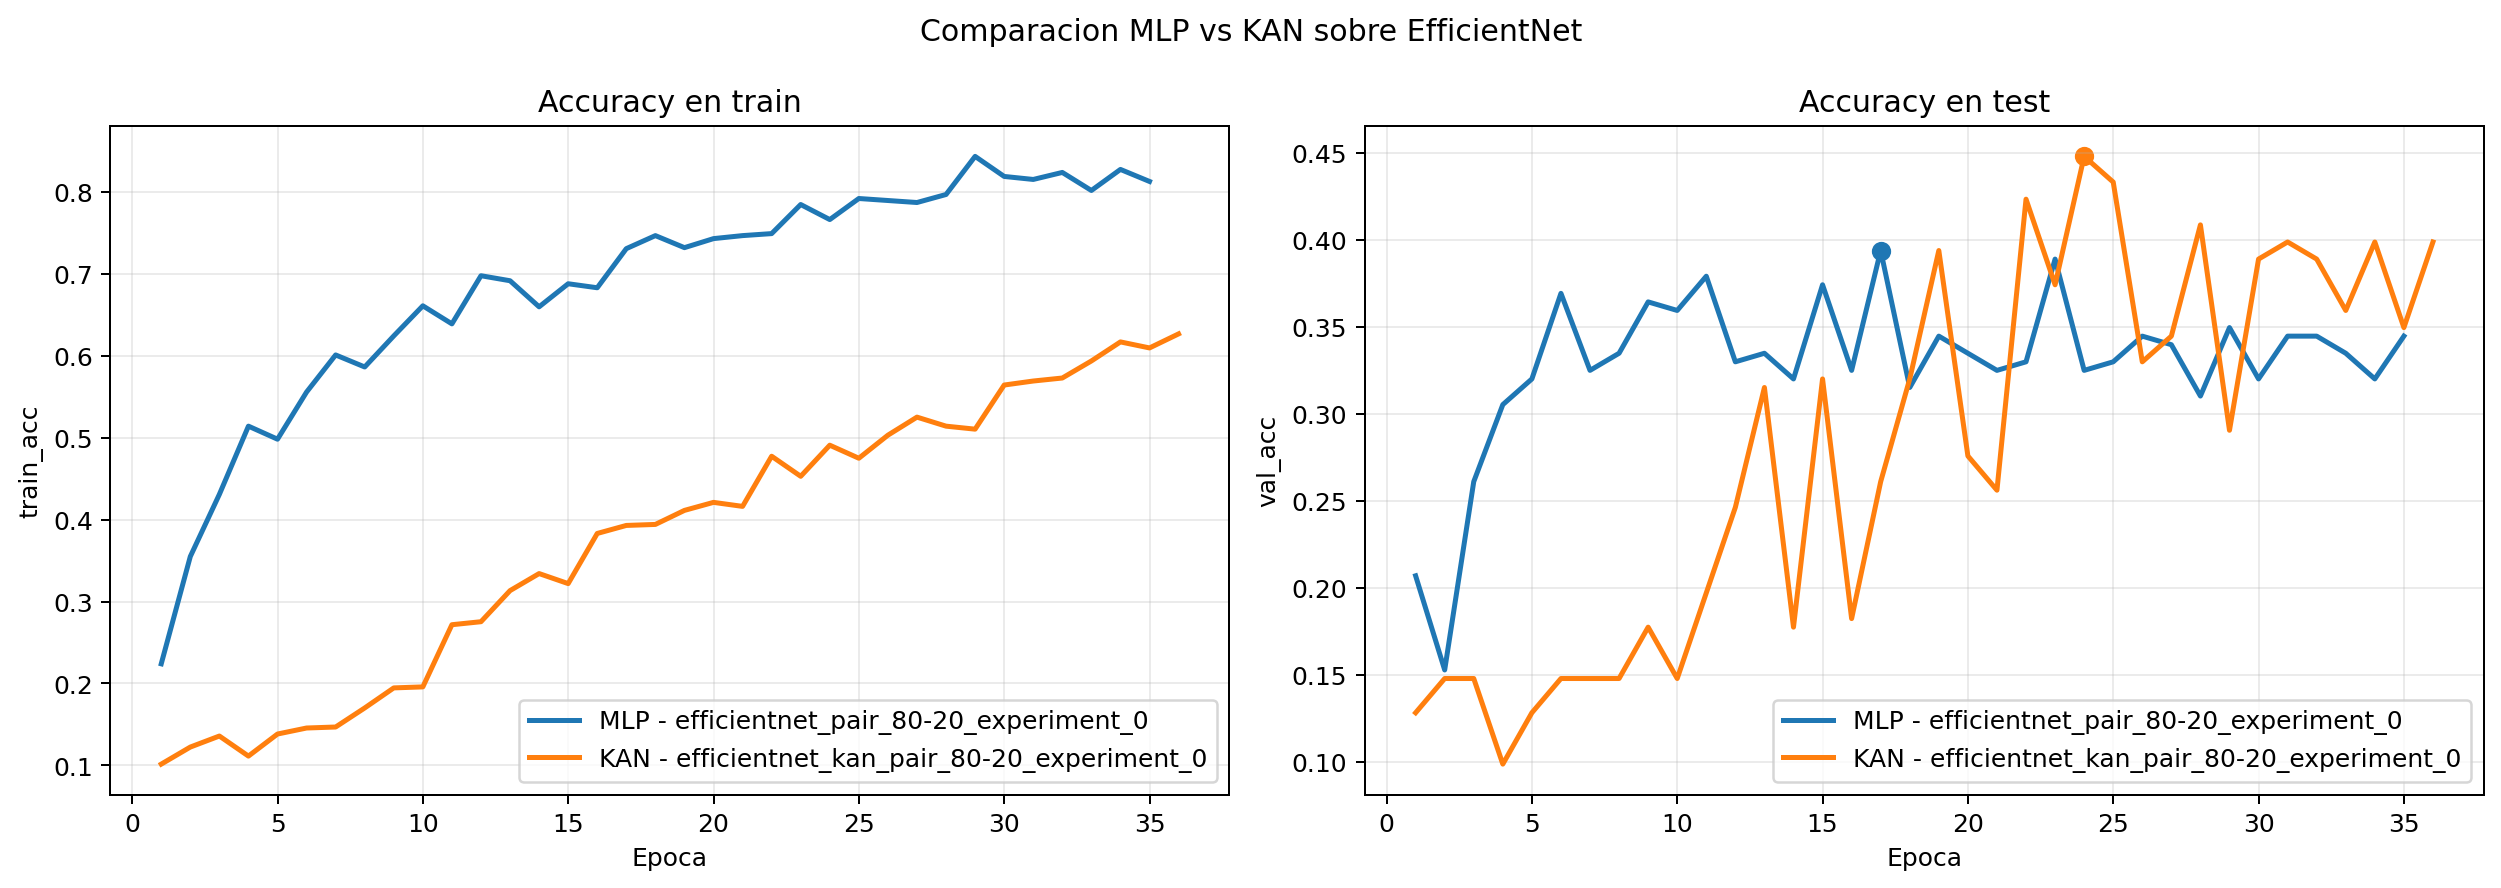
\includegraphics[width=\linewidth]{efficientnet_comparacion_mlp_kan.png}
    \caption{Curvas de \texttt{train\_acc} y \texttt{val\_acc}.}
\end{subfigure}

\vspace{0.8cm}

\begin{subfigure}[t]{0.82\textwidth}
    \centering
    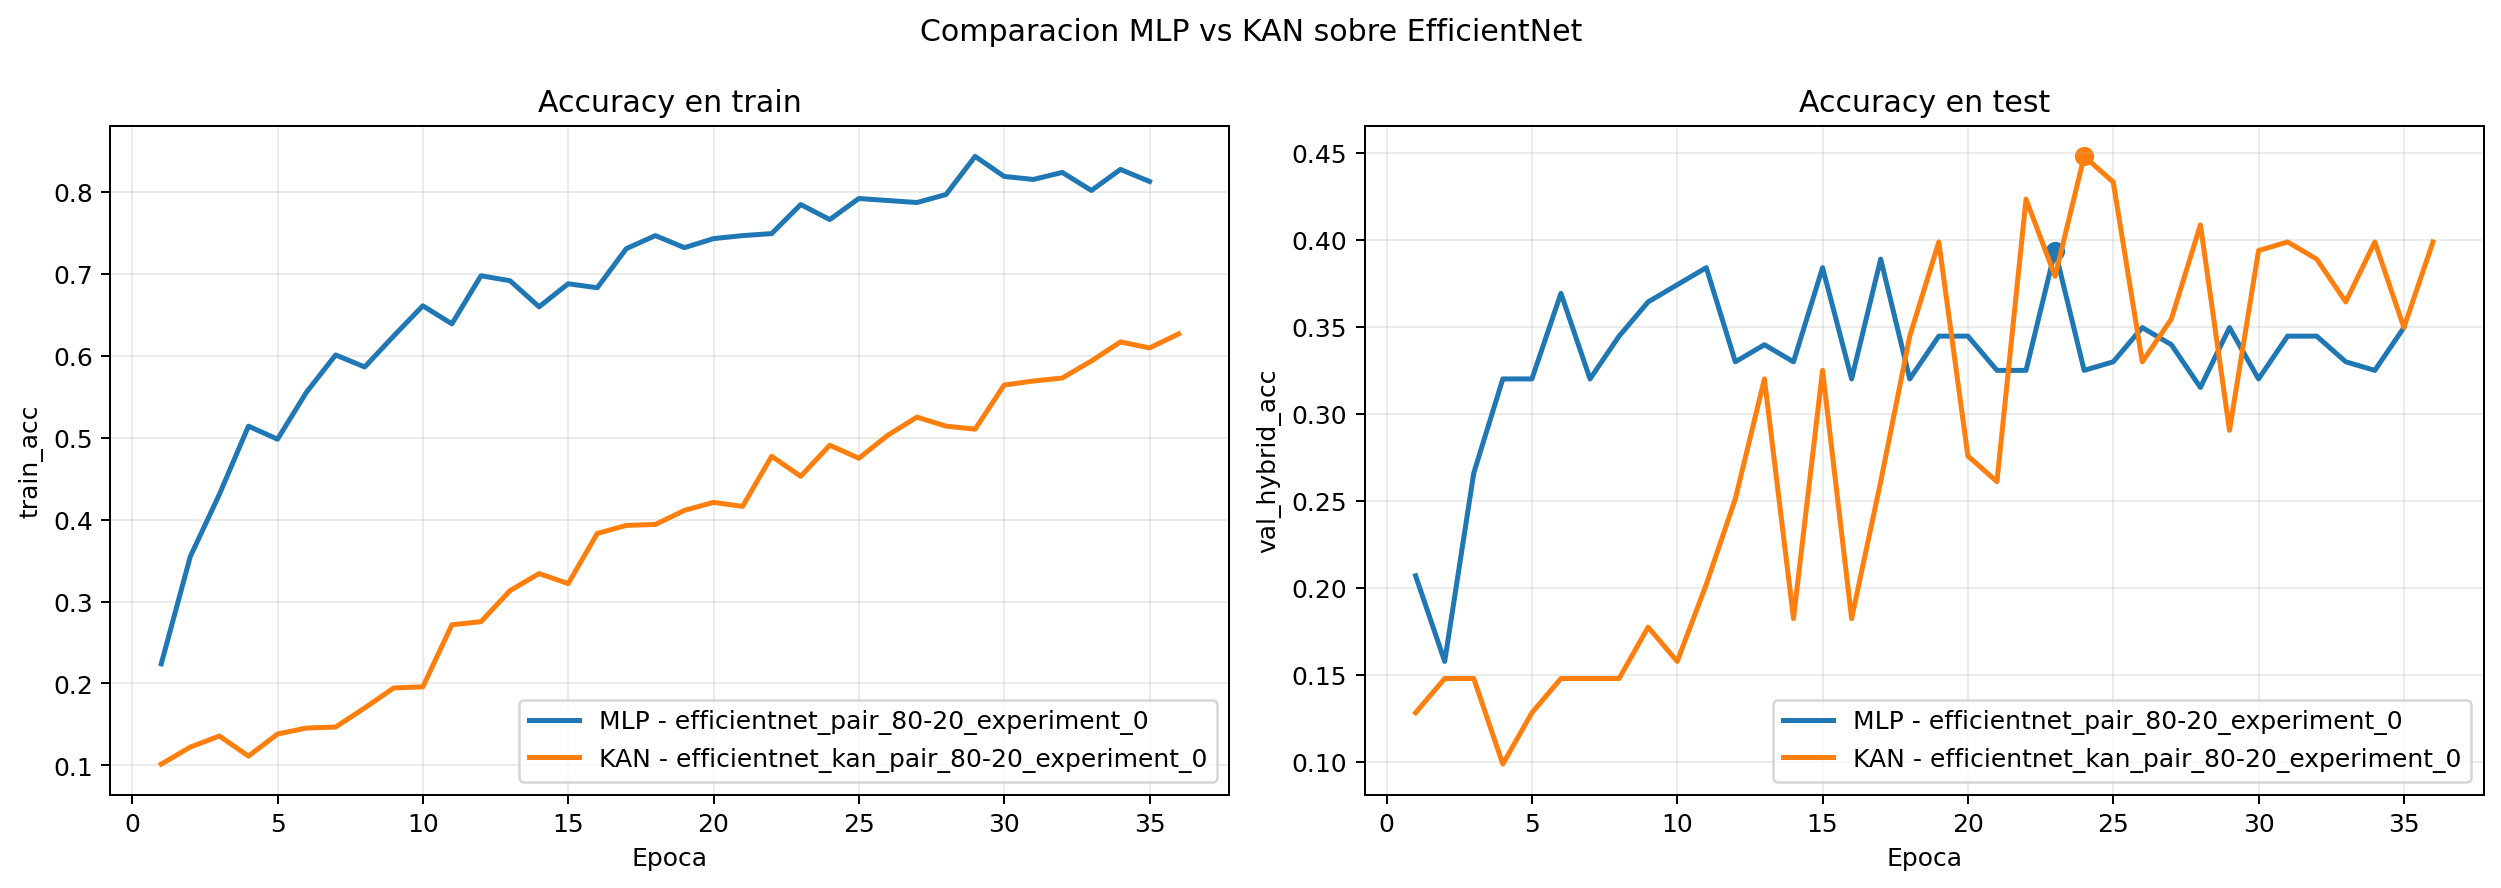
\includegraphics[width=\linewidth]{efficientnet_comparacion_mlp_kan_hybrid.png}
    \caption{Curvas de \texttt{train\_acc} y \texttt{val\_hybrid\_acc}.}
\end{subfigure}
\caption{Comparaci\'on de las curvas de aprendizaje para las dos cabezas finales sobre \texttt{EfficientNet}.}
\label{fig:efficientnet-curvas}
\end{figure}

Las curvas de la Figura~\ref{fig:efficientnet-curvas} apoyan esta lectura. La cabeza MLP alcanza niveles de entrenamiento m\'as altos, pero sus curvas de validaci\'on se estabilizan antes y en un nivel inferior. La cabeza KAN progresa de forma m\'as gradual y consigue una validaci\'on final m\'as alta y m\'as consistente.

\section{An\'alisis visual de ejemplos}

Para complementar la comparaci\'on num\'erica se generaron mosaicos de ejemplos del conjunto de test. Las Figuras~\ref{fig:efficientnet-mosaico-mlp} y~\ref{fig:efficientnet-mosaico-kan} permiten inspeccionar cualitativamente el comportamiento de ambas variantes sobre ocho pares representativos.

\clearpage

\begin{figure}[p]
\centering
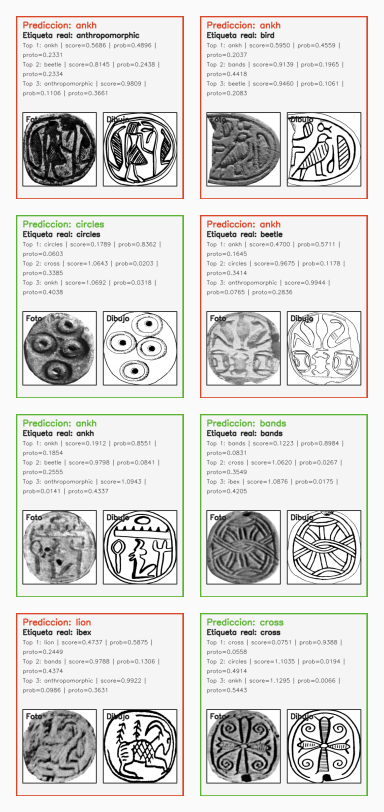
\includegraphics[width=\textwidth,height=0.86\textheight,keepaspectratio]{efficientnet_mlp_mosaico_resumen.png}
\caption{Resumen visual de \texttt{EfficientNet + MLP}.}
\label{fig:efficientnet-mosaico-mlp}
\end{figure}

\begin{figure}[p]
\centering
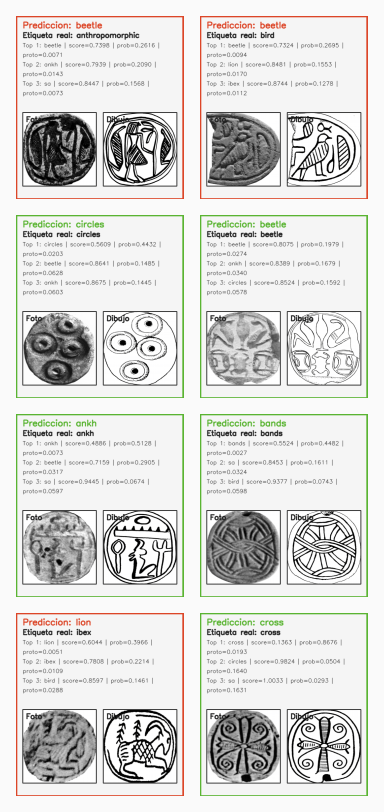
\includegraphics[width=\textwidth,height=0.86\textheight,keepaspectratio]{efficientnet_kan_mosaico_resumen.png}
\caption{Resumen visual de \texttt{EfficientNet + KAN}.}
\label{fig:efficientnet-mosaico-kan}
\end{figure}

\clearpage

Estos mosaicos no sustituyen a la evaluaci\'on cuantitativa, pero ayudan a interpretar el tipo de errores. En la selecci\'on mostrada, la variante MLP acierta 4 de 8 ejemplos, mientras que la variante KAN acierta 5 de 8. Ambos modelos comparten algunas confusiones sem\'anticas, por ejemplo entre \texttt{ibex} y \texttt{lion}, lo que sugiere que ciertas formas siguen siendo ambiguas incluso cuando se combinan fotograf\'ia y dibujo.

Sin embargo, tambi\'en se aprecian diferencias cualitativas. La variante KAN corrige al menos uno de los fallos que el modelo MLP comet\'ia en esta misma selecci\'on, como el ejemplo cuyo artefacto real es \texttt{beetle}. En cambio, ambos siguen fallando en algunos casos donde la similitud geom\'etrica entre clases es alta, especialmente en ejemplos con rasgos compartidos o con informaci\'on visual menos discriminativa.

\section{Discusi\'on del segundo bloque}

La comparaci\'on sobre \texttt{EfficientNet} cambia la lectura obtenida en el primer bloque. Cuando se parte de un backbone potente y preentrenado y solo se modifica el bloque final de clasificaci\'on, la cabeza KAN s\'i muestra una ventaja emp\'irica frente a la MLP. Esto sugiere que la expresividad adicional de KAN puede ser m\'as \'util cuando el extractor de caracter\'isticas ya proporciona embeddings ricos y relativamente estables.

Dicho de otro modo, en el primer bloque la limitaci\'on principal parec\'ia estar en la representaci\'on. En el segundo bloque, esa representaci\'on la aporta \texttt{EfficientNet}, de modo que la diferencia entre MLP y KAN se vuelve m\'as visible. En este contexto, la KAN parece aprovechar mejor el espacio de embeddings fusionado foto+dibujo y produce una frontera de decisi\'on m\'as adecuada para el problema.

\section{Conclusi\'on general}

Los dos bloques del trabajo llevan a una conclusi\'on matizada. En modelos ligeros, especialmente cuando interviene un VAE y el volumen de datos es reducido, la KAN no ha mostrado una mejora consistente sobre la MLP. Sin embargo, al pasar a un escenario de \textit{transfer learning} con \texttt{EfficientNet-B0}, la situaci\'on cambia: manteniendo fijo el backbone y variando solo la cabeza final, la variante KAN obtiene mejores resultados que la variante MLP tanto en accuracy directa como en la m\'etrica h\'ibrida.

En conjunto, esto sugiere que las capas KAN no deben evaluarse aisladamente, sino en funci\'on de la calidad de la representaci\'on sobre la que operan. En este proyecto, su ventaja aparece con mayor claridad cuando trabajan sobre embeddings de alto nivel extra\'idos por un backbone preentrenado. Por ello, la comparaci\'on \texttt{EfficientNet + MLP/KAN} constituye un resultado m\'as favorable para KAN que el observado en el bloque inicial de arquitecturas ligeras.

\end{document}
